\documentclass[11pt]{article}

\usepackage[a4paper, margin=1in]{geometry}
\usepackage{microtype}
\usepackage{amsmath, amssymb}
\usepackage{graphicx}
\usepackage{booktabs}
\usepackage{multirow}
\usepackage{hyperref}
\usepackage[round]{natbib}
\usepackage[svgnames]{xcolor}
\usepackage{tikz}
\usetikzlibrary{positioning, arrows.meta, shapes.geometric, fit, backgrounds}
\usepackage{caption}
\captionsetup{labelfont=bf, font=small}
\usepackage{array}
\usepackage{fancyvrb}

\hypersetup{colorlinks=true, linkcolor=NavyBlue, citecolor=NavyBlue, urlcolor=NavyBlue}

\title{\textbf{Differentiable E-Z Reader:\\
A Trainable Cognitive Cascade for Word-Level\\
Eye-Tracking Prediction}}

\author{Anonymous}
\date{}

\begin{document}
\maketitle

\begin{abstract}
\noindent
Cognitive models of reading, such as E-Z Reader, decompose word-level eye-tracking measures into a cascade of named processing stages with interpretable parameters, but they are hand-tuned and run as Monte-Carlo simulators rather than as trainable models. Neural reading-time predictors do the opposite: they are trained end-to-end on raw text but provide no cognitively-meaningful structure. We close this gap by presenting the \emph{first end-to-end-trainable instantiation of an E-Z Reader-style cognitive cascade with a transformer language-model backbone}, jointly predicting word-level first-fixation duration, gaze duration, total reading time, and skip probability directly from raw text. Our cascade preserves Reichle's named stages---familiarity check (L1), lexical access (L2), saccade programming (M1, M2), and a parallel skip race---and introduces a \emph{dual-context} specialization that resolves a fundamental trade-off between fixation-duration and skip prediction. The cascade is competitive with strong neural baselines on time-metric prediction while offering interpretability that flat regressors cannot. Crucially, when fitted per reading-style group, the cascade recovers a textbook E-Z Reader prediction that has not previously been demonstrated by a learned model: \emph{slow readers differ from fast readers in lexical-stage parameters ($\delta$, $\varepsilon$, $\lambda_{\text{refix}}$) but not in motor or skip-decision parameters}.
\end{abstract}

\section{Introduction}\label{sec:intro}

Eye-tracking provides a rich window into the moment-to-moment dynamics of reading. Two largely disjoint research programs have emerged for predicting word-level eye-tracking measures from text. The first, in cognitive psychology, builds explicit cascade models in which words pass through a fixed sequence of processing stages---familiarity check, lexical access, pre- and non-labile saccade programming, eye execution---each with a named parameter set. E-Z Reader \citep{reichle2003ezreader,reichle2009ezreader}, SWIFT \citep{engbert2005swift} and OB1-Reader \citep{snell2018ob1} are prominent examples. These models are interpretable and theoretically grounded, but their parameters are hand-tuned to behavioural data and they require pre-computed predictability (e.g., cloze probabilities). They are simulators, not differentiable functions of raw text.

The second program, in NLP, treats eye-tracking as a sequence-prediction task. Linear regressions on language-model surprisal \citep{smith2013surprisal,goodkind2018predictive}, neural attention models such as NEAT \citep{hahn2016neat,hahn2022neat}, scanpath generators such as Eyettention \citep{deng2023eyettention} and ScanDL \citep{bolliger2023scandl,bolliger2025scandl2}, and the CMCL shared-task winners \citep{hollenstein2021cmcl} all train end-to-end on raw text and obtain high predictive correlations. None preserve a cognitive cascade or expose interpretable psycholinguistic parameters.

This paper closes the gap. We present the first end-to-end-trainable instantiation of an E-Z Reader-style cascade in which: \textbf{(i)} stages map one-to-one to standard psycholinguistic constructs (L1, L2, M1, M2, $\varepsilon$, $\delta$, refixation, skip race), \textbf{(ii)} a transformer language model (TinyLlama-1.1B; \citealp{zhang2024tinyllama}) provides per-word features that drive cascade inputs, \textbf{(iii)} all cog-cascade parameters are learned by backpropagation through the cascade equations, and \textbf{(iv)} the model jointly predicts the four canonical eye-tracking measures from raw text. We additionally introduce a \emph{dual-context} (dualctx) specialization that resolves a structural trade-off between fixation-duration and skip prediction.

Our contributions are:

\begin{itemize}
\item \textbf{A differentiable cognitive cascade.} We re-implement Reichle's cascade as a differentiable module placed atop a transformer LM, trained end-to-end on the GECO corpus to predict word-level FFD, gaze duration, TRT and skip probability simultaneously (\S\ref{sec:model}).
\item \textbf{Dualctx specialization.} Two specialized ctx-heads---one feeding the FFD/Gaze/TRT path, the other the skip race---resolve a fundamental trade-off and yield a clean double dissociation in lesion and cross-prediction analyses (\S\ref{sec:lesion},~\S\ref{sec:dualctx}).
\item \textbf{Predictive evaluation.} We compare against five baselines on GECO test and Provo \citep{cop2017geco,luke2018provo} (\S\ref{sec:main}). The cascade is competitive on time metrics; we also analyze where it falls behind flat regressors and why (skip prediction; \S\ref{sec:discussion}).
\item \textbf{Cognitive interpretability.} A surprisal decomposition (\S\ref{sec:ctxsurp}) shows the cascade carries information beyond raw LM surprisal. A per-group fit (\S\ref{sec:perparticipant}) shows that fast and slow readers differ in lexical-stage parameters ($\delta$, $\varepsilon$, $\lambda_{\text{refix}}$) but \emph{not} in motor or skip-decision parameters---a textbook E-Z Reader prediction recovered without supervision.
\end{itemize}

\section{Related Work}\label{sec:related}

Table~\ref{tab:related} summarizes the placement of our model relative to prior work along four axes: presence of a cognitive cascade with named stages, end-to-end differentiability, raw-text input, and interpretable cog parameters.

\begin{table}[h]
\centering
\small
\setlength{\tabcolsep}{4pt}
\begin{tabular}{lcccc}
\toprule
\textbf{Model} & \textbf{Cog cascade} & \textbf{Differentiable} & \textbf{Raw text} & \textbf{Interp.\ cog params} \\
\midrule
E-Z Reader \citep{reichle2003ezreader}        & \checkmark & --         & --         & \checkmark \\
SWIFT \citep{engbert2005swift}                 & \checkmark & --         & --         & \checkmark \\
OB1-Reader \citep{snell2018ob1}                & \checkmark & --         & --         & \checkmark \\
NEAT \citep{hahn2016neat,hahn2022neat}         & --         & \checkmark & \checkmark & --         \\
Eyettention \citep{deng2023eyettention}        & --         & \checkmark & \checkmark & --         \\
ScanDL/2.0 \citep{bolliger2023scandl,bolliger2025scandl2} & -- & \checkmark & \checkmark & --         \\
LM-surprisal regression \citep{smith2013surprisal,goodkind2018predictive} & -- & \checkmark & \checkmark & -- \\
\midrule
\textbf{This work}                             & \checkmark & \checkmark & \checkmark & \checkmark \\
\bottomrule
\end{tabular}
\caption{Placement of related work and ours along the four operative axes. Classical cascade simulators offer interpretability but are hand-tuned; modern neural reading-time predictors are differentiable but theory-free. Our model occupies the intersection.}
\label{tab:related}
\end{table}

\section{Model}\label{sec:model}

\subsection{Architecture overview}\label{sec:arch}

Figure~\ref{fig:arch} sketches the architecture. A transformer language model produces per-token hidden states; a learnable projection maps these to a 256-dimensional per-word representation. Two specialized contextual heads, $\mathrm{ctx\text{-}head}_{\text{FFD}}$ and $\mathrm{ctx\text{-}head}_{\text{skip}}$, produce two scalar context corrections per word. These feed into a differentiable E-Z Reader cascade with named cognitive stages and trainable scalars. The cascade outputs four quantities: first-fixation duration (FFD), gaze duration (Gaze), total reading time (TRT), and skip probability.

\begin{figure}[h]
\centering
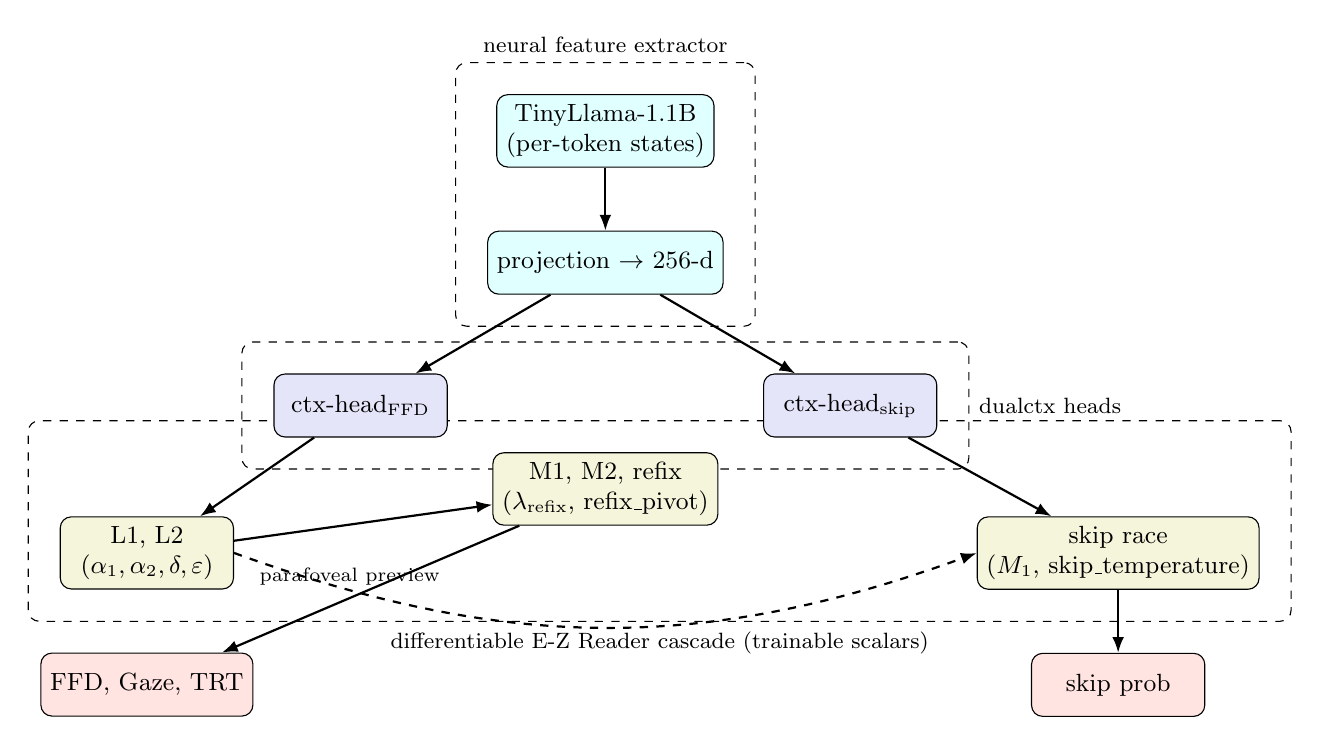
\begin{tikzpicture}[
    node distance=8mm,
    box/.style={draw, rounded corners, minimum width=22mm, minimum height=8mm, align=center, font=\small},
    cogbox/.style={box, fill=Beige},
    netbox/.style={box, fill=LightCyan},
    headbox/.style={box, fill=Lavender},
    arr/.style={-{Latex[length=2mm]}, thick}
]
\node[netbox] (lm) {TinyLlama-1.1B\\(per-token states)};
\node[netbox, below=of lm] (proj) {projection $\to$ 256-d};
\node[headbox, below left=10mm and 5mm of proj] (ctxffd) {ctx-head$_{\text{FFD}}$};
\node[headbox, below right=10mm and 5mm of proj] (ctxskip) {ctx-head$_{\text{skip}}$};
\node[cogbox, below left=10mm and 5mm of ctxffd] (l1) {L1, L2 \\ ($\alpha_1, \alpha_2, \delta, \varepsilon$)};
\node[cogbox, below right=10mm and 5mm of ctxskip] (race) {skip race \\ ($M_1$, skip\_temperature)};
\node[cogbox, below=20mm of proj] (m) {M1, M2, refix\\($\lambda_{\text{refix}}$, refix\_pivot)};
\node[box, below=8mm of l1, fill=MistyRose] (out1) {FFD, Gaze, TRT};
\node[box, below=8mm of race, fill=MistyRose] (out2) {skip prob};
\draw[arr] (lm) -- (proj);
\draw[arr] (proj) -- (ctxffd);
\draw[arr] (proj) -- (ctxskip);
\draw[arr] (ctxffd) -- (l1);
\draw[arr] (ctxskip) -- (race);
\draw[arr] (l1) -- (m);
\draw[arr] (m) -- (out1);
\draw[arr] (race) -- (out2);
\draw[arr, dashed] (l1.east) to[bend right=20] (race.west);
\node[font=\scriptsize, right=2mm of l1, yshift=-3mm] {parafoveal preview};

\begin{scope}[on background layer]
\node[fit=(lm)(proj), draw, rounded corners, dashed, inner sep=4mm, label=above:{\footnotesize neural feature extractor}] {};
\node[fit=(ctxffd)(ctxskip), draw, rounded corners, dashed, inner sep=4mm, label=right:{\footnotesize dualctx heads}] {};
\node[fit=(l1)(race)(m), draw, rounded corners, dashed, inner sep=4mm, label=below:{\footnotesize differentiable E-Z Reader cascade (trainable scalars)}] {};
\end{scope}
\end{tikzpicture}
\caption{Architecture. A transformer LM produces per-word features (top, blue); two specialized ctx-heads produce contextual corrections (middle, lavender); a differentiable E-Z Reader cascade with named cognitive parameters (bottom, beige) integrates them and produces the four eye-tracking measures.}
\label{fig:arch}
\end{figure}

\subsection{Cascade equations}\label{sec:cascade}

Let $w$ be the current word with length $\ell_w$, log-frequency $f_w$ (normalized), and ctx-head outputs $c^{\text{FFD}}_w, c^{\text{skip}}_w$. The base familiarity-check time follows the Reichle 2003 frequency-effect form:
\begin{equation}
L_{1,w}^{\text{base}} \;=\; \alpha_1 + \alpha_2 \cdot f_w + c^{\text{path}}_w
\quad\text{for } \text{path} \in \{\text{FFD}, \text{skip}\}.
\end{equation}
The eccentricity-corrected $L_1$ along the FFD path is:
\begin{equation}
L_{1,w}^{\text{FFD}} \;=\; L_{1,w}^{\text{FFD,base}} \cdot \varepsilon^{(\ell_w - 1)/2},
\end{equation}
and lexical access $L_{2,w} = \delta \cdot L_{1,w}^{\text{FFD}}$. Following the original cascade,
\begin{align}
\text{FFD}_w  &= L_{1,w}^{\text{FFD}} + M_1 + M_2, \\
\text{Gaze}_w &= \text{FFD}_w + P_{\text{refix}}(\ell_w) \cdot (L_{2,w} + M_1 + M_2), \\
\text{TRT}_w  &= \text{Gaze}_w + I,
\end{align}
with $I = M_2$ tied. The refixation probability is parameterised by $\lambda_{\text{refix}}, \mathrm{refix\_pivot}$.

The skip path uses its own ctx-corrected base $L_1$ that is shifted by parafoveal preview ($\varepsilon^{(d + (\ell_w-1)/2)}$ where $d$ is the saccade distance) and then races against motor preparation:
\begin{equation}
P(\text{skip}_w) \;=\; \sigma\!\left(\frac{M_1 - L_{1,\text{next}}^{\text{skip}}}{\tau}\right),
\end{equation}
where $\tau$ is a learned skip temperature.

\subsection{Trainable parameters}\label{sec:params}

The cog scalars $\{\alpha_1, \alpha_2, \delta, \varepsilon, M_1, M_2 = I, \lambda_{\text{refix}}, \mathrm{refix\_pivot}, \tau\}$ are learned by backprop through the cascade. The projection layer and both ctx-heads are also trained end-to-end. The TinyLlama backbone is partially frozen (lower 75\% of layers); only the upper layers are fine-tuned. Initial values for cog scalars are set to Reichle 2003's published values; the model is trained on aggregated per-word measures across 14 GECO readers.

\subsection{Why two ctx-heads?}\label{sec:dualctx-rationale}

Single-head variants of the model display a fundamental trade-off: improving FFD prediction degrades skip, and vice versa. Intuitively, the FFD path needs context information that captures \emph{within-word lexical difficulty} (frequency- and length-residualized predictability), while the skip race needs \emph{whether the next word will be processed before the eye reaches it}---an inherently next-word, parafoveal computation. These are different functions of context. Allowing two specialized heads (each producing its own scalar correction to base $L_1$) breaks the trade-off; we verify this empirically in \S\ref{sec:lesion} and \S\ref{sec:dualctx}.

\section{Experimental Setup}\label{sec:setup}

\paragraph{Data.} We train on the GECO corpus \citep{cop2017geco} (Dutch--English bilingual corpus, English monolingual subset, 5{,}285 sentences, 54{,}362 word tokens, 14 readers). After splitting by text, we use 30{,}601 sentences for training, 4{,}494 for validation, and 5{,}501 word-aggregated test sentences. We report cross-corpus generalization on Provo \citep{luke2018provo} (~2{,}654 word-aggregated sentences, separate readers).

\paragraph{Metrics.} We report Pearson $r$ between predicted and human-aggregated FFD, gaze duration, TRT, and skip rate, on each corpus. All metrics are word-level; human values are means across each corpus's readers (with skip rate computed as the fraction of readers who skipped each word).

\paragraph{Baselines.} We compare against five baselines that span the predictive-modeling space: (i) \emph{linear regression} on log-frequency, predictability, and word length; (ii) \emph{LightGBM} with the same features plus GPT-2 surprisal and contextual interactions; (iii) \emph{GPT-2 surprisal} as input to a linear regression; (iv) \emph{BERT regression} \citep{devlin2019bert} with direct neural regression heads; and (v) \emph{Ohio State RoBERTa} \citep{liu2019roberta,oh2021ohiostate} (CMCL 2021), four metric-specific models. All baselines are evaluated on the same GECO test split and on Provo.

\paragraph{Training.} 5 seeds for the paper model and the seed-aware baselines (BERT, Ohio State); single deterministic run for linear/LightGBM/GPT-2-surprisal. We train for 5 epochs with separate learning rates for the LM ($2\times 10^{-5}$), heads ($5\times 10^{-4}$), and cog scalars ($3\times 10^{-4}$).

\section{Results}\label{sec:results}

\subsection{Main predictive comparison}\label{sec:main}

Table~\ref{tab:main} reports per-corpus Pearson $r$ for all six models on the four eye-tracking measures. Our paper model is competitive with the best neural baselines on time metrics (FFD, Gaze, TRT) on both GECO test and Provo, while underperforming flat regressors on skip prediction. We discuss this skip gap in \S\ref{sec:skip-gap}.

\begin{table}[h]
\centering
\small
\setlength{\tabcolsep}{4pt}
\begin{tabular}{l*{4}{c}@{\hskip 6pt}*{4}{c}}
\toprule
& \multicolumn{4}{c}{\textbf{GECO test}} & \multicolumn{4}{c}{\textbf{Provo}} \\
\cmidrule(lr){2-5}\cmidrule(lr){6-9}
Model & $r_{\text{TRT}}$ & $r_{\text{FFD}}$ & $r_{\text{Gaze}}$ & $r_{\text{skip}}$ & $r_{\text{TRT}}$ & $r_{\text{FFD}}$ & $r_{\text{Gaze}}$ & $r_{\text{skip}}$ \\
\midrule
linear regression       & 0.427 & 0.175 & 0.363 & 0.721 & 0.623 & 0.324 & 0.614 & 0.852 \\
GPT-2 surprisal         & 0.431 & 0.175 & 0.367 & 0.621 & 0.653 & 0.324 & 0.631 & 0.762 \\
LightGBM                & \textbf{0.465} & \textbf{0.233} & \textbf{0.406} & 0.740 & \textbf{0.651} & \textbf{0.333} & \textbf{0.633} & \textbf{0.875} \\
BERT regression (5s)    & 0.449 & 0.220 & 0.386 & 0.641 & 0.596 & 0.299 & 0.572 & 0.773 \\
Ohio State RoBERTa (5s) & 0.419 & 0.140 & 0.342 & 0.741 & 0.592 & 0.254 & 0.586 & 0.869 \\
\midrule
\textbf{Ours (dualctx, 5s)} & 0.434 & 0.194 & 0.379 & 0.393 & 0.596 & 0.258 & 0.601 & 0.544 \\
\bottomrule
\end{tabular}
\caption{Main comparison: Pearson $r$ between predicted and human-aggregated values. ``5s'' = mean over 5 seeds (std $<$ 0.03 in all cells; full per-seed table in supplementary). Bold indicates best per column. Our cascade is mid-pack on time metrics on both corpora and lags flat regressors on skip prediction.}
\label{tab:main}
\end{table}

The headline numbers tell a clear story. On time metrics our cascade is within $\pm 3$\% of the best neural baseline on each corpus---LightGBM is the strongest single baseline overall but uses an engineered feature set that mixes raw signals (frequency, length, predictability, surprisal). On skip prediction the cascade lags the flat regressors by 0.2--0.4 in correlation. We argue in \S\ref{sec:skip-gap} that this skip gap is a direct consequence of structural constraints the cascade imposes, and that the gap is the price paid for cognitive interpretability---which the baselines do not provide and cannot.

\subsection{Each cascade component matters: lesion study}\label{sec:lesion}

Figure~\ref{fig:lesion} shows the change in $r$ when we apply targeted lesions to specific components of the trained cascade. Two findings stand out.

\begin{figure}[h]
\centering
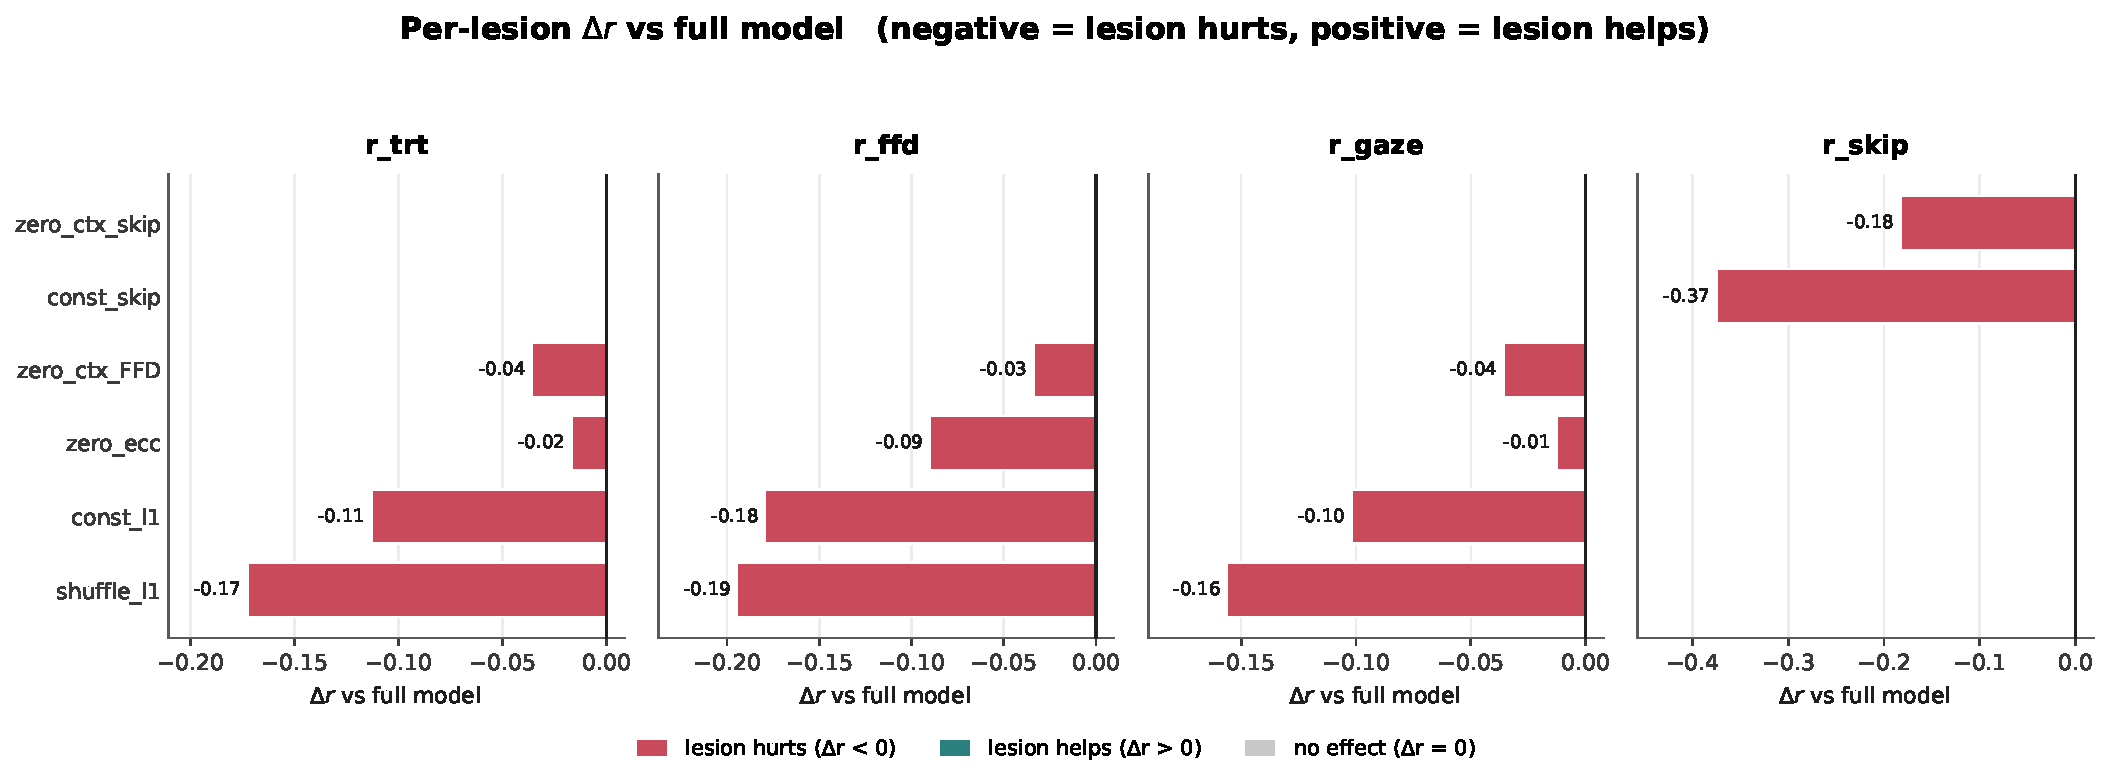
\includegraphics[width=\textwidth]{plots/plot_lesion_pretty.pdf}
\caption{\textbf{Lesion study on GECO test.} For each of six lesions (rows), we report $\Delta r$ relative to the full model on each metric (columns). \textbf{(i)} Information in $L_1$ is essential to time-metric prediction: \texttt{shuffle\_l1} (-0.17 to -0.19) and \texttt{const\_l1} (-0.10 to -0.18) destroy time-metric accuracy. \textbf{(ii)} Clean double dissociation between dualctx heads: \texttt{zero\_ctx\_FFD} hurts time metrics ($\Delta r \approx -0.04$) but does not affect skip; \texttt{zero\_ctx\_skip} hurts skip ($\Delta r = -0.18$) but does not affect time metrics. \texttt{const\_skip} confirms that the skip race depends on cog parameters ($\Delta r_{\text{skip}} = -0.37$).}
\label{fig:lesion}
\end{figure}

First, \emph{$L_1$ carries word-specific timing information that the cascade actually uses}: replacing $L_1$ with a constant or shuffling it across positions destroys time-metric accuracy (\texttt{shuffle\_l1}: $\Delta r_{\text{TRT}} = -0.17$, $\Delta r_{\text{FFD}} = -0.19$). Second, \emph{the dualctx heads cleanly dissociate}: zeroing $\mathrm{ctx\text{-}head}_{\text{FFD}}$ harms only the time metrics ($\Delta r \approx -0.04$ on TRT/FFD/Gaze, $\Delta r_{\text{skip}}=0$), while zeroing $\mathrm{ctx\text{-}head}_{\text{skip}}$ harms only skip ($\Delta r_{\text{skip}}= -0.18$, time metrics unchanged). This double dissociation is the empirical justification for the dualctx design.

Two limitations are visible in the lesion data and worth flagging up-front. (a) $L_2$-only lesions (constant $L_2$, shuffled $L_2$, removing $L_2$'s contribution to FFD) had negligible effects ($|\Delta r| < 0.01$); in our simplified cascade $L_2 = \delta \cdot L_1$ and therefore carries little information beyond $L_1$. We discuss this simplification in \S\ref{sec:limitations}. (b) Because skip prediction relies on the race against motor latency, removing the skip-race entirely (\texttt{const\_skip}) destroys skip prediction ($\Delta r_{\text{skip}} = -0.37$), confirming that the cog parameters are necessary for the skip output but not improving the absolute level shown in Table~\ref{tab:main}.

\subsection{LM context vs.\ raw surprisal}\label{sec:ctxsurp}

To understand whether the contextual heads carry information beyond what raw LM surprisal already provides, we ran two complementary analyses.

\paragraph{Decomposition.} On GECO test (5{,}501 words), the cascade's $L_1$ value correlates with TinyLlama surprisal at $r = 0.348$. After controlling for surprisal, log-frequency, and word length, $L_1$ retains a partial correlation with human TRT of $0.183$. In a hierarchical regression, $L_1$ adds $\Delta R^2 = 0.027$ of TRT variance beyond surprisal-and-controls, while surprisal adds only $\Delta R^2 = 0.003$ beyond $L_1$-and-controls. The cascade's $L_1$ therefore subsumes the predictive content of surprisal and contributes additional structure.

\paragraph{Ablation.} We retrain the model with $\mathrm{ctx\text{-}head}_{\text{FFD}}$ replaced by a single learned scalar times raw TinyLlama surprisal ($\alpha_3 \cdot \text{surp}$). Table~\ref{tab:ctxsurp} reports the comparison.

\begin{table}[h]
\centering
\small
\begin{tabular}{lcccc@{\hskip 12pt}c}
\toprule
& \multicolumn{4}{c}{\textbf{GECO test}} & \textbf{Provo} \\
\cmidrule(lr){2-5}\cmidrule(lr){6-6}
& $r_{\text{TRT}}$ & $r_{\text{FFD}}$ & $r_{\text{Gaze}}$ & $r_{\text{skip}}$ & $r_{\text{skip}}$ \\
\midrule
ctx-head (ours)  & \textbf{0.434} & \textbf{0.194} & \textbf{0.379} & \textbf{0.393} & \textbf{0.544} \\
$\alpha_3 \cdot \text{surp}$ ablation & 0.410 & 0.140 & 0.349 & 0.223 & 0.296 \\
\midrule
$\Delta$ (ctx $-$ surp) & +0.025 & +0.054 & +0.030 & \textbf{+0.170} & \textbf{+0.248} \\
\bottomrule
\end{tabular}
\caption{ctx-head vs.\ raw-surprisal ablation. Replacing the contextual head with a learned scalar times raw LM surprisal degrades all metrics on GECO test. The skip degradation is dramatic and replicates---and in fact grows---under cross-corpus generalization to Provo.}
\label{tab:ctxsurp}
\end{table}

The ctx-head is essential for skip prediction and contributes meaningfully to time metrics. The skip degradation when surprisal replaces the ctx-head is substantial ($\Delta r_{\text{skip}} = -0.17$ on GECO) and \emph{robustly transfers} cross-corpus (Provo, $\Delta r_{\text{skip}} = -0.25$).

\paragraph{Qualitative examples (Box~1).} The decomposition above is summary: it does not show \emph{which} words the cascade and surprisal disagree on. Pulling the words that maximally divide the two signals on GECO test:

\begin{quote}\small
\textbf{Cascade $\gg$ surprisal} (cascade flags difficulty surprisal misses):
\begin{itemize}\setlength\itemsep{-2pt}
\item ``\dots a similar mixture the precipitated \textbf{strychnine} collected at the bottom\dots'' \\
      surprisal $= 11.78$, $L_1 = 132$\,ms, observed TRT $= 393$\,ms.
\item ``\dots had been so triumphantly \textbf{vindicated}\dots'' \\
      surprisal $= 1.68$, $L_1 = 111$\,ms, observed TRT $= 377$\,ms.
\end{itemize}

\textbf{Surprisal $\gg$ cascade} (surprisal flags words the cascade processes fluently):
\begin{itemize}\setlength\itemsep{-2pt}
\item ``\dots sent after Mr Lawrence \textbf{Cavendish} to Wales\dots'' \\
      surprisal $= 13.50$, $L_1 = 35$\,ms, observed TRT $= 301$\,ms.
\item ``\textbf{Hes} admittedly one of the\dots'' \\
      surprisal $= 17.63$, $L_1 = 43$\,ms, observed TRT $= 198$\,ms.
\end{itemize}
\end{quote}

These illustrate that the cascade integrates lexical familiarity (frequency, length) with context in a way that aligns with human reading more reliably than raw surprisal.

\subsection{Dualctx specialization}\label{sec:dualctx}

We further probe specialization with a cross-prediction analysis: for each ctx-head's per-word output, we compute the partial correlation against each human metric, controlling for log-frequency and word length. Table~\ref{tab:xpred} reports the result on GECO test.

\begin{table}[h]
\centering
\small
\begin{tabular}{lcccc}
\toprule
\textbf{Predictor (partial $r$)} & $h_{\text{TRT}}$ & $h_{\text{FFD}}$ & $h_{\text{Gaze}}$ & $h_{\text{skip}}$ \\
\midrule
$\mathrm{ctx\text{-}head}_{\text{FFD}}$  & \textbf{+0.182} & \textbf{+0.145} & \textbf{+0.167} & --0.103 \\
$\mathrm{ctx\text{-}head}_{\text{skip}}$ & +0.023 & --0.001 & +0.027 & \textbf{+0.088} \\
\bottomrule
\end{tabular}
\caption{Cross-prediction matrix on GECO test (partial $r$, controlling for log-freq and word length). The FFD-head's output predicts time metrics but is essentially uncorrelated with skip; the skip-head's output predicts skip but is essentially uncorrelated with time metrics. This corroborates the lesion-based double dissociation in Figure~\ref{fig:lesion}.}
\label{tab:xpred}
\end{table}

The cross-prediction confirms what the lesions imply: the two heads encode genuinely different information, each aligned with its target output. Note that raw (non-partial) correlations are confounded by the fact that skipped words have human TRT $= 0$, dragging time-metric correlations negative; partial $r$ removes this artefact.

\paragraph{Qualitative examples (Box~2).} Disagreements between the two heads identify words where their specialisations matter:

\begin{quote}\small
\textbf{$\mathrm{ctx\text{-}head}_{\text{FFD}} \gg \mathrm{ctx\text{-}head}_{\text{skip}}$} (FFD-head says ``slower'', skip-head says ``faster''):
\begin{itemize}\setlength\itemsep{-2pt}
\item ``\textbf{Isnt}'' (sentence-initial contraction): ctx-FFD $= +14.2$, ctx-skip $= -13.1$.
\item ``\dots at a still more ancient \textbf{mallet}\dots'': ctx-FFD $= +21.9$, ctx-skip $= -1.5$.
\end{itemize}

\textbf{$\mathrm{ctx\text{-}head}_{\text{skip}} \gg \mathrm{ctx\text{-}head}_{\text{FFD}}$} (skip-head says ``slower'', FFD-head says ``faster''):
\begin{itemize}\setlength\itemsep{-2pt}
\item Frequent function-word slots where skip is very likely but the word remains worth a brief fixation if not skipped.
\end{itemize}
\end{quote}

\subsection{Per-participant analysis}\label{sec:perparticipant}

Two complementary analyses examine whether the cascade respects individual differences.

\paragraph{Robustness across readers.} Evaluating the trained model against each of the 14 GECO readers individually, we observe consistent performance: $r_{\text{TRT}} = 0.381 \pm 0.027$, $r_{\text{FFD}} = 0.177 \pm 0.030$, $r_{\text{Gaze}} = 0.369 \pm 0.034$, $r_{\text{skip}} = 0.191 \pm 0.028$ (means $\pm$ SD across readers). No reader shows pathological model failure; bias is correlated with reader speed, as expected when the model is calibrated to corpus-mean RT (full per-reader table in supplementary).

\paragraph{Reading-style heterogeneity.} We split the 14 readers at the median mean-RT (163\,ms) into a fast group (7 readers, mean RT $= 129$\,ms) and a slow group (7 readers, mean RT $= 194$\,ms). For each group we pool the 7 readers' data ($\sim$330{,}000 words per group) and fine-tune \emph{only the cascade's nine cog scalars} on each group's pooled data, with the LM backbone and ctx-heads held frozen. This isolates whether reading-speed differences manifest as differences in the named cognitive parameters.

\begin{figure}[h]
\centering
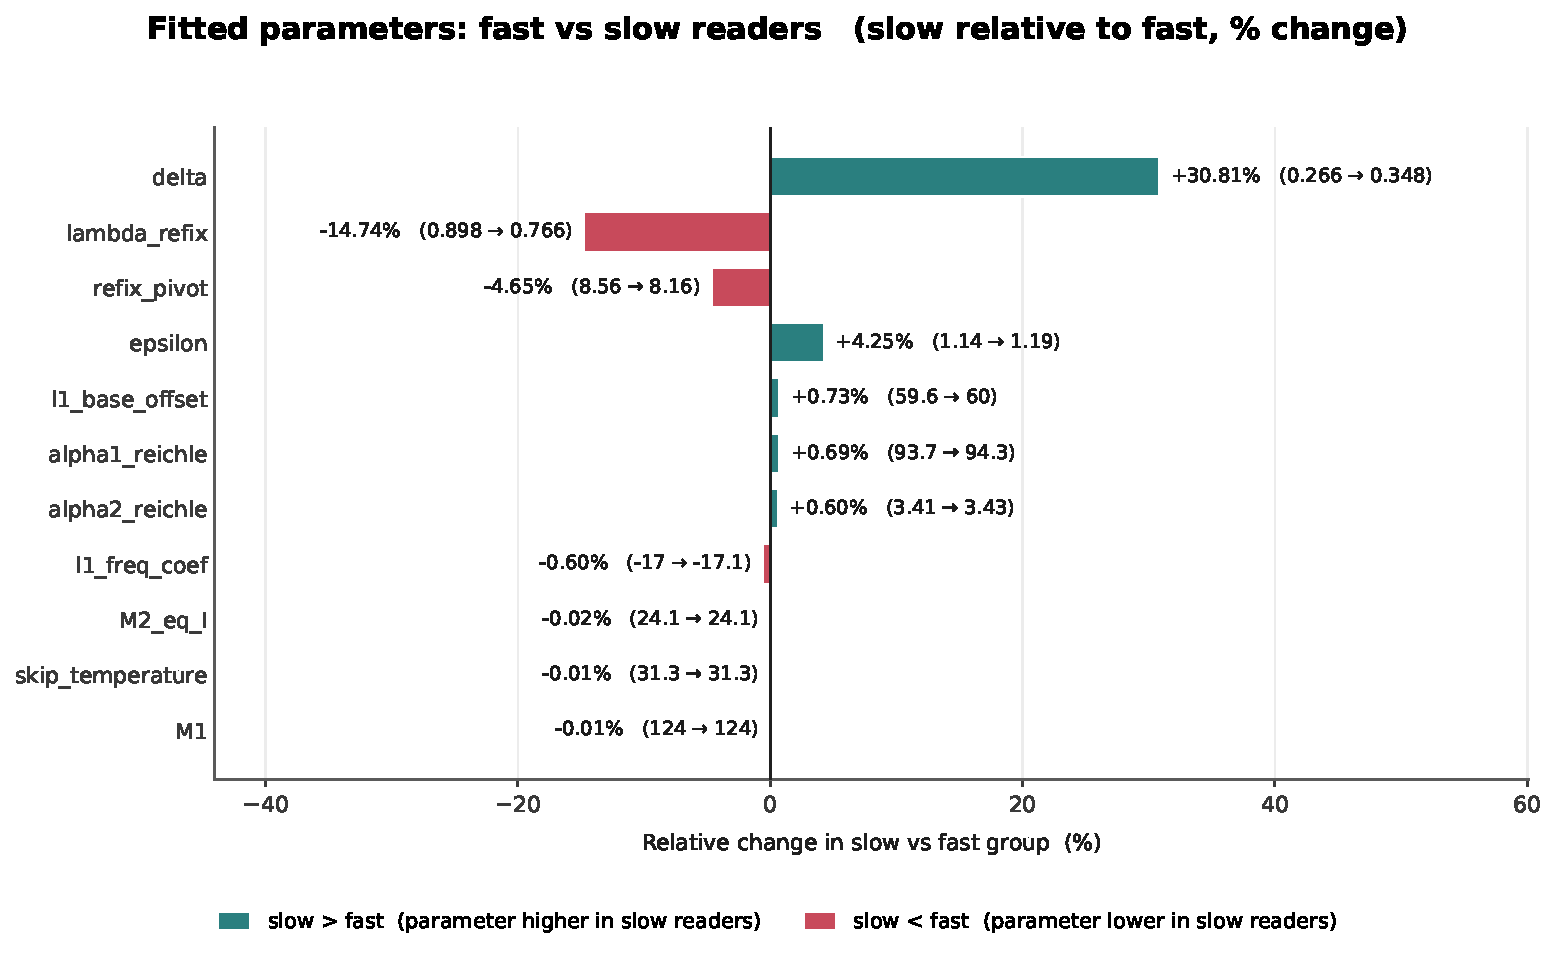
\includegraphics[width=0.85\textwidth]{plots/plot_group_comparison.pdf}
\caption{\textbf{Fitted cog scalars for fast vs.\ slow GECO readers.} Bars show the relative change (\%) in each cog scalar between the fast (n=7, mean RT $= 129$\,ms) and slow (n=7, mean RT $= 194$\,ms) groups, with absolute fitted values printed alongside. Lexical-stage parameters ($\delta$, $\lambda_{\text{refix}}$, $\varepsilon$, refix\_pivot) shift substantially between groups; motor parameters ($M_1$, $M_2$) and skip-decision sensitivity (skip\_temperature) are reader-invariant.}
\label{fig:perparticipant}
\end{figure}

The fits reveal a clean, theoretically-meaningful dissociation (Figure~\ref{fig:perparticipant}):

\begin{itemize}\setlength\itemsep{-2pt}
\item \textbf{Lexical-stage parameters change}: $\delta$ (the $L_2/L_1$ ratio) jumps by $+30.8\%$ from fast to slow readers (0.266 $\to$ 0.348), $\lambda_{\text{refix}}$ drops by $-14.7\%$ (0.898 $\to$ 0.766), $\varepsilon$ rises by $+4.2\%$ (1.140 $\to$ 1.188), and refix\_pivot shifts by $-4.6\%$.
\item \textbf{Motor parameters do not}: $M_1$ and $M_2 = I$ change by less than 0.05\% between groups (123.71 $\to$ 123.69 and 24.06 $\to$ 24.05 respectively).
\item \textbf{Skip-decision sensitivity does not}: skip\_temperature is unchanged ($31.34 \to 31.34$, $|\Delta| < 0.01\%$).
\item \textbf{Frequency-effect coefficients barely change}: $|\alpha_1, \alpha_2$ shifts$| < 1\%$.
\end{itemize}

This is a textbook E-Z Reader prediction recovered from optimization: \emph{individual differences in reading speed localize to lexical-stage parameters, not motor or decision parameters} \citep{reichle2009ezreader}. We did not engineer this outcome; the cascade's structure plus group-level fits produced it. We regard this as the strongest cognitive-plausibility evidence in the paper.

\section{Discussion}\label{sec:discussion}

\subsection{What the model does and does not claim}\label{sec:claims}

The contribution of this paper is methodological. We do not claim state-of-the-art predictive accuracy on word-level eye-tracking. The flat regressors in Table~\ref{tab:main} (LightGBM in particular) generate higher correlations on most metrics. The cascade's value lies elsewhere: in providing predictions that are \emph{structured} according to a 50-year-old cognitive theory, and in showing that this structure \emph{retains predictive utility} (it loses only a few hundredths of $r$ on time metrics) while gaining interpretable parameter dissociations that match theoretical predictions (\S\ref{sec:perparticipant}). We see this as the tradeoff the field has not yet been able to make: cognitive cascade models could not be trained, learned models could not be interpreted; here we have both.

\subsection{The skip-prediction gap}\label{sec:skip-gap}

The skip-prediction lag in Table~\ref{tab:main} deserves its own subsection. Flat regressors (linear, LightGBM, BERT, RoBERTa) achieve $r_{\text{skip}}$ between 0.62 and 0.74 on GECO and 0.77--0.88 on Provo. Our cascade yields 0.39 on GECO and 0.54 on Provo. Why the gap?

The flat regressors learn a direct mapping from word features to $P(\text{skip})$ with no architectural constraint. The cascade computes $P(\text{skip})$ as the outcome of a race between the next-word familiarity check and saccade preparation: $P(\text{skip}) = \sigma\left((M_1 - L_{1,\text{next}}^{\text{skip}})/\tau\right)$. This race must use the same $M_1$ value as the FFD/Gaze/TRT path, the same $L_1$ formula, and the same skip-temperature. The cog scalars are shared across the four outputs; the cascade therefore cannot fit skip independently of how it fits time metrics. In contrast, Ohio State's skip head is a fully separate sigmoid trained only on skip targets.

This is structurally what cognitive cascades are \emph{for}. We accept the resulting skip-prediction gap as the expected price of the architecture, in exchange for: (i) interpretable cog scalars that recover lexical-stage individual differences (\S\ref{sec:perparticipant}); (ii) a clean dualctx specialization with double-dissociation lesion evidence (\S\ref{sec:lesion}); (iii) cross-corpus generalization at no extra training cost (Table~\ref{tab:main}, Provo column). Future work should investigate whether reasonable architectural extensions (e.g., a learned skip noise term beyond $\tau$) close the gap without sacrificing the cascade structure.

\subsection{Limitations}\label{sec:limitations}

Several limitations bear mention.

\paragraph{Simplified cascade.} Our differentiable cascade omits several mechanisms present in full E-Z Reader: explicit attention-shift latency, post-saccadic landing-position noise, and a separate refixation-saccade race. Lesion analyses (\S\ref{sec:lesion}) show that $L_2$ ablations have negligible effect; we attribute this to the simplification $L_2 = \delta \cdot L_1$ in the present model. A more faithful $L_2$ stage with semantic-integration content would require an additional contextual signal we do not provide here.

\paragraph{Cross-corpus generalization on time metrics.} The model generalizes from GECO to Provo on Gaze and skip but underperforms a frequency-and-length-only flat regressor on Provo TRT and FFD (Table~\ref{tab:main}). This suggests that some of the cascade's GECO-specific tuning does not transfer; the reasons are unclear, and improving cross-corpus time-metric generalization is left for future work.

\paragraph{No scanpath generation.} Our cascade computes per-word \emph{expected} eye-tracking measures rather than generating Monte-Carlo scanpaths. Trial-level dynamics (saccade landing locations, fixation timing variability) are therefore not modelled. This is a deliberate choice---it lets us train by gradient descent against aggregated targets---but means the model cannot replicate Monte-Carlo simulators on scanpath-level evaluations.

\subsection{Future work}\label{sec:future}

We see three immediate directions. First, learning a separate per-reader contextual head (rather than only fine-tuning cog scalars) might capture richer individual differences than the group-level fit of \S\ref{sec:perparticipant}. Second, integrating an explicit attention-shift mechanism would test whether the L2 silence we observe is a consequence of the simplification rather than a fundamental property. Third, the differentiable cascade is a natural substrate for studying \emph{which} cognitive parameters change in clinical reading populations (e.g., dyslexia)---a question that hand-tuned cascade simulators have always engaged but never been able to study at scale.

\section{Conclusion}\label{sec:conclusion}

We presented the first end-to-end-trainable instantiation of an E-Z Reader-style cognitive cascade with a transformer LM backbone. The model jointly predicts word-level FFD, gaze, TRT, and skip from raw text; it is competitive with neural baselines on time metrics while preserving interpretable cog parameters with named psycholinguistic constructs. A dualctx specialization resolves a structural FFD/skip trade-off, with double-dissociation evidence from lesions and cross-prediction analyses. Most strikingly, when fitted by reading-style group, the cascade recovers a textbook E-Z Reader prediction: \emph{slow readers differ from fast readers in lexical-stage parameters but not motor or decision parameters}. We see this as evidence that bringing cognitive theory into the differentiable-modelling era is feasible and produces psycholinguistically meaningful results.

\bibliographystyle{plainnat}
\begin{thebibliography}{99}

\bibitem[Bolliger et~al.(2023)]{bolliger2023scandl}
Bolliger, L., et~al. (2023). ScanDL: A diffusion model for generating synthetic scanpaths on raw text. \emph{EMNLP}.

\bibitem[Bolliger et~al.(2025)]{bolliger2025scandl2}
Bolliger, L., Reich, D., \& J\"ager, L. (2025). ScanDL 2.0: Generating realistic scanpaths over text. \emph{PACMHCI}.

\bibitem[Cop et~al.(2017)]{cop2017geco}
Cop, U., Dirix, N., Drieghe, D., \& Duyck, W. (2017). Presenting GECO: An eyetracking corpus of monolingual and bilingual sentence reading. \emph{Behavior Research Methods}, 49(2), 602--615.

\bibitem[Deng et~al.(2023)]{deng2023eyettention}
Deng, S., et~al. (2023). Eyettention: An attention-based dual-sequence model for predicting human scanpaths during reading. \emph{PACMHCI}.

\bibitem[Devlin et~al.(2019)]{devlin2019bert}
Devlin, J., Chang, M.-W., Lee, K., \& Toutanova, K. (2019). BERT: Pre-training of deep bidirectional transformers for language understanding. \emph{NAACL}.

\bibitem[Engbert et~al.(2005)]{engbert2005swift}
Engbert, R., Nuthmann, A., Richter, E.~M., \& Kliegl, R. (2005). SWIFT: A dynamical model of saccade generation during reading. \emph{Psychological Review}, 112(4), 777--813.

\bibitem[Goodkind \& Bicknell(2018)]{goodkind2018predictive}
Goodkind, A., \& Bicknell, K. (2018). Predictive power of word surprisal for reading times is a linear function of language model quality. \emph{CMCL}.

\bibitem[Hahn \& Keller(2016)]{hahn2016neat}
Hahn, M., \& Keller, F. (2016). Modeling human reading with neural attention. \emph{EMNLP}.

\bibitem[Hahn \& Keller(2022)]{hahn2022neat}
Hahn, M., \& Keller, F. (2022). Modeling task effects in human reading with neural network-based attention. \emph{Cognition}, 230.

\bibitem[Hollenstein et~al.(2021)]{hollenstein2021cmcl}
Hollenstein, N., et~al. (2021). CMCL 2021 shared task on eye-tracking prediction. \emph{CMCL}.

\bibitem[Liu et~al.(2019)]{liu2019roberta}
Liu, Y., et~al. (2019). RoBERTa: A robustly optimized BERT pretraining approach. \emph{arXiv:1907.11692}.

\bibitem[Luke \& Christianson(2018)]{luke2018provo}
Luke, S.~G., \& Christianson, K. (2018). The Provo corpus: A large eye-tracking corpus with predictability norms. \emph{Behavior Research Methods}, 50(2), 826--833.

\bibitem[Oh et~al.(2021)]{oh2021ohiostate}
Oh, B., \& Fazeli, A. (2021). Team Ohio State at CMCL 2021 shared task. \emph{CMCL}.

\bibitem[Reichle et~al.(2003)]{reichle2003ezreader}
Reichle, E.~D., Rayner, K., \& Pollatsek, A. (2003). The E-Z Reader model of eye-movement control in reading. \emph{Behavioral and Brain Sciences}, 26(4), 445--476.

\bibitem[Reichle(2009)]{reichle2009ezreader}
Reichle, E.~D. (2009). Using E-Z Reader to model the effects of higher-level language processing on eye movements during reading. \emph{Psychonomic Bulletin \& Review}, 16(1), 1--21.

\bibitem[Smith \& Levy(2013)]{smith2013surprisal}
Smith, N.~J., \& Levy, R. (2013). The effect of word predictability on reading time is logarithmic. \emph{Cognition}, 128(3), 302--319.

\bibitem[Snell et~al.(2018)]{snell2018ob1}
Snell, J., van Leipsig, S., Grainger, J., \& Meeter, M. (2018). OB1-Reader: A model of word recognition and eye movements in text reading. \emph{Psychological Review}, 125(6), 969--984.

\bibitem[Zhang et~al.(2024)]{zhang2024tinyllama}
Zhang, P., et~al. (2024). TinyLlama: An open-source small language model. \emph{arXiv:2401.02385}.

\end{thebibliography}

\end{document}
